Here, we define the proposed model of computation. We start with a brief, informal description. Then, we will provide formal definitions and discuss their connections to AADL syntax and semantics.

A system consists of components, connections between components, and a schedule.
Every component is associated with two Boolean variables \emph{dispatch} and \emph{complete}.
The schedule defines the time of dispatch, and the time of completion of each component within a scheduling cycle.
A component is activated when it is dispatched.
Component activation ends when it is completed.
A valid schedule is one where component activations do not overlap.
%Once a component is activated, it runs to complete. There is no preemption.
A component reads input at dispatch time. %Reading is non-blocking. It reads the most recent input data value or an initial value. 
And the input is \emph{frozen} during the component activation.
A component writes output at completion time. %Writing is non-blocking. It overwrites the previous data value. 
And the output holds its data value between its completions.
%The connections represent an asynchrnous communication channel with a buffer of size one.
The connections between components are unidirectional. It represents communication through shared variable with one writer and possible multiple readers. 
A component checks its input assumptions at dispatch time. %If the assumption is violated, then the system is consided \emph{inconsistent}.
A component ensures its guarantees at completion time. 

{\bf signal.}
A signal $x$ is a function of the form $x: N \mapsto T_x$, where $N$ is the set of natural numbers including zero, and $T_x$ is the data type of $x(i)$ for all $i \in N$.
$x(i)$, an assignment of a vlaue in $T_x$ to $x$, is called a \emph{valuation} of signal $x$. A signal represents a possibly infinite sequence of values.
The data type can be either a primitive data type (e.g. real, bool, int, and enumeration types) or a composite data type (e.g. record types). 
%Assume the data type of signal $x$ and $y$ is $T_x$ and $T_y$, respectively, $x = y$ means that $T_x=T_y$ and $x_i = y_i$ for all $i \in N$. 

{\bf port.}
Input ports $X = \{x_1, x_2, ... x_M\}$, where $x_i$ is the \emph{i}-th input port, and $M$ is the total number of input ports. Each port $x \in X$ is uniquely associated with a signal. We may use input port or input signal interchangablely. To simplify the notation, we use the port ID $x$ to denote the associated \emph{signal}. Outputs are defined similarly. 

We model the AADL ports as signals. In particular, an event port is modelled as a sequence of Boolean values. %The value \emph{true} or \emph{false} indicates an event is \emph{present} or \emph{absent} at the port, respectively. 
An event data port is modelled as a pair of data signal and event signal. We use the port name $p$ to denote its associated data signal, and $event(p)$ to denote its associated event signal. 

{\bf component.}
A component is a eight-tuple $(S, s_0, I, O, \delta, A, P, clock)$, where 
\begin{itemize}
    	\item $S$ is a finite non-empty set of states;
    	\item $s_0 \in S$ is the initial state;
    	\item $I$ is a set of input signals valuations;
    	\item $O$ is a set of output signals valuations;
    	\item $\delta$ is the state transfer function of the form $\delta: I \times S \mapsto S$;
    	\item $A$ is a set of \emph{assumptions}, for all $a \in A$, $a$ is a Boolan function $I \times S \mapsto B$;
    	\item $P$ is a set of \emph{gurarantees}, for all $p \in P$, $p$ is a Boolan function $I \times O \times S \mapsto B$;
	\item $clock$ is a Boolean signal $clock(n+1) \Rightarrow \lnot clock(n+2) \land  \lnot clock(n), \forall i \in N$ .
\end{itemize}

%$\lambda$ is the output relation of the form $\lambda: (I,S) \mapsto O$. 
Let $s: N \mapsto S$, we have $ s(n+1) = \delta (s(n), I(n))$ 
%and $ O(n) = \delta (s(n), I(n))$, 
where $I(n) = \{x_1(n), x_2(n), ... x_N(n)\}$, for all $n \in N$. 
  
%The ports of a thread are divided into two finite disctinct sets: input ports ($I$) and output ports ($O$). Correspondingly, the associated signals are divided int to input signals and output signals. We model the \emph{state} of a thread with a finite set $S$ of signals. %The next state function is $T: S x I \mapsto S'$. The output function is $T: S x I \mapsto S$. Then, a thread is %A thread is modelled as a collection of input signals and output signals. A thread could be aossciated with /emph{local} states, which are not accessible outside the scope of the thread. They are modelled as signals, noted as set S . 

{\bf component execution.}

%A component is associated with two Boolean signals (events) \emph{dispatch} ($d$) and \emph{complete} ($c$). A component is \emph{dispatched} at time $i$, if and only if $d(i) = true$. A component is \emph{complete} at time $i$, if and only if $c(i) = true$. %A component can be in either \emph{active} or \emph{sleep} mode. 
%At \emph{dispatch} a component evaluates the inputs. At \emph{complete}, it updates its output and transitions to its \emph{next state}. After \emph{complete}, it holds its state and output till next \emph{complete}. That is,

An valuation of an assumption $a$ at time $n$ is $a(n) =  a(I(n), s(n))$. 
An valuation of a gurarantee $p$ at time $n$ is $p(n) =  p(I(n), O(n), s(n))$. 

At \emph{clock}, the \emph{assumptions} $A$ should hold. That is,
$$d(i) \Rightarrow a_i, \forall i\in N, \forall a \in A $$
If it is violated, the component is inconsistent.

At \emph{clock}, the \emph{gurarantees} $P$ should hold. That is,
$$clock(n) \Rightarrow p(n), \forall n\in N, \forall p \in P $$

A compoent holds its state and output between \emph{clock}. That is,
$$\lnot clock(n) \Rightarrow y(n+1) = y(n), \forall n \in N, \forall y \in Y$$
$$\lnot clock(n) \Rightarrow s(n+1) = s(n), \forall n \in N, \forall s \in S$$



%The \emph{dispatch} and \emph{complete} models, respectively, the start and end of the time slot that a component to run. 
%When its \emph{dispatch} event $d$ is present, a thread samples the input values and starts execution. This is the time when the associated AGREE \emph{assumptions} $A$ should hold. That is,
%$$event(d)_i \Rightarrow a_i, \forall i\in N, \forall a \in A $$

{\bf connection.}
A \emph{connection} from an output port $y \in Y$ of one component $C$ to an input port $x' \in X'$ of another component $C'$ implies the corresponding signals $x' = y$.
Define intial input

%An AADL \emph{connection} between an input port $i$ of one thread and an output port $o$ of another thread enforces the equality of their associated signals. For data ports, this means $i = o$. For event data prots, this means $i = o$ and $event(i) = event(o)$. %For simplicity, we define $e(p) = false^*$ if $p$ is a data port.

%{\bf virtual events.}
%We introduce two virtual input event ports: \emph{dispatch} ($d$) and \emph{complete} ($c$) for each thread.  The \emph{dispatch} and \emph{complete} event models, respectively, the start and end of the time slot that a scheduler allocated to a thread to run. 
%{\bf thread execution.}
%When its \emph{dispatch} event $d$ is present, a thread samples the input values and starts execution. 

%When its \emph{complete} event $c$ is present, a thread updates its ouput signal $o$ value, otherwise it holds its previous value. That is, 
The output hold combined with the definition of \emph{connection} models the asynchronous communication. It could be viewed as a shared variable, which has one writer and possibly multiple readers. Since under our MoC, at most one component is active at a time, there is no ambiguity on the order of read and write actions. It also could be viewed as a buffer (or queue) of size one. It overwrites when overflow occurs. Note that, unlike synchronous dataflow models, the data (\emph{token}) is not disgarded after \emph{consumption}. That is, reading is non-destroying. This ensures that in case of \emph{upsampling}, the consumer samples the same input value repeatedly. 

{\bf AGREE contracts.}
A component is associated with a set of AGREE \emph{assumptions} $A$ and \emph{gurarantees} $P$, where $a \in A$ is a Boolan function $(I, S) \mapsto B$, $p \in P$ is a Boolan function $(I, O, S) \mapsto B$. The evaluation of assumption $a$ at time $i$ is denoted as $a_i$. The evaluation of gurarantee $p$ at time $i$ is denoted as $p_i$. 
	
At \emph{dispatch}, the \emph{assumptions} $A$ should hold. That is,
$$d(i) \Rightarrow a_i, \forall i\in N, \forall a \in A $$

At \emph{complete}, the \emph{gurarantees} $P$ should hold. That is,
$$c(i) \Rightarrow p_i, \forall i\in N, \forall p \in P $$
%Here we assume a thread always completes its execution within the assigned time slot. Thus, there is no pre-emption. 

%We denote the initial value of a signal as $x_0$. For an event port $p$, $e(p_0) = false$. The output write action is also non-blocking. In other words, a thread will not halt its execution due to waiting for an previous output data to be \emph{consumed}. It overwrites.

Figure \ref{wpmAGREE} shows an exmaple of how the proposed MoC could be modelled in the AGREE annex.

\begin{figure}[ht!]
\centering
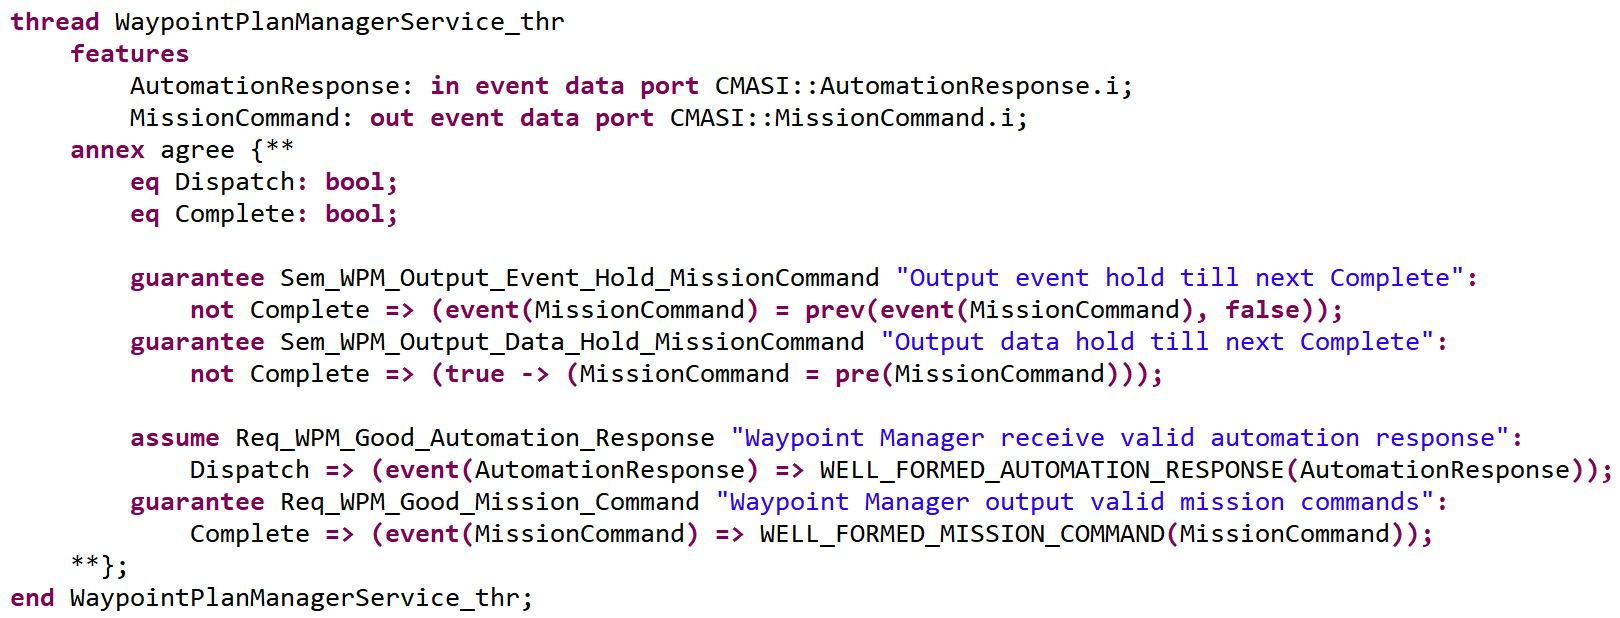
\includegraphics[width=120mm]{wpmAGREE.jpg}
\caption{An AGREE Model Example\label{wpmAGREE}}
\end{figure}

{\bf schedule.}
Given a finite set of components $C = \{c_1, c_2,... C_N\}$, where $c_i$ is the \emph{i}-th component, a schedule is a set of triple $(c_i, dispatch, complete)$.
A schedule $\sigma$ defines when a component out of a set of components $P$ is activated. That is,  
$$\sigma = \{(p, d, c), \forall p \in P  \}$$ 
We assume schedules are static, periodic, and valid. A schedule is called valid if in each period or \emph{cycle}, there is no other scheduling event between any pair of \emph{dispatch} and \emph{complete} of the same component, and the \emph{dispatch} event occurs before the matching \emph{complete} event. 

In a schedule model, one has to choose the mapping from a \emph{tick} to physical time. A tick could be the basic time unit, or a common divisor. For example, given a schedule with a period of 10 ms, starting with component A 4 ms, idle 2 ms, component B 2 ms, idle 2 ms, then a model of the schedule could be $\sigma = \{d(A)=(1,0,0,0,0)^*, c(A) = (0,0,1,0,0)^*, d(B) = (0,0,0,1,0)^*, c(B) = (0,0,0,0,1)^*\}$, where each \emph{tick} models 2 ms. 

We introduce a circular counter to model a schedule in AGREE. The counter updates at each tick. The maximum count models the period of the schedule. An AGREE model of the schedule $(ABACD)^*$ used in the example is shown in Figure \ref{schedule}.
\begin{figure}[ht!]
\centering
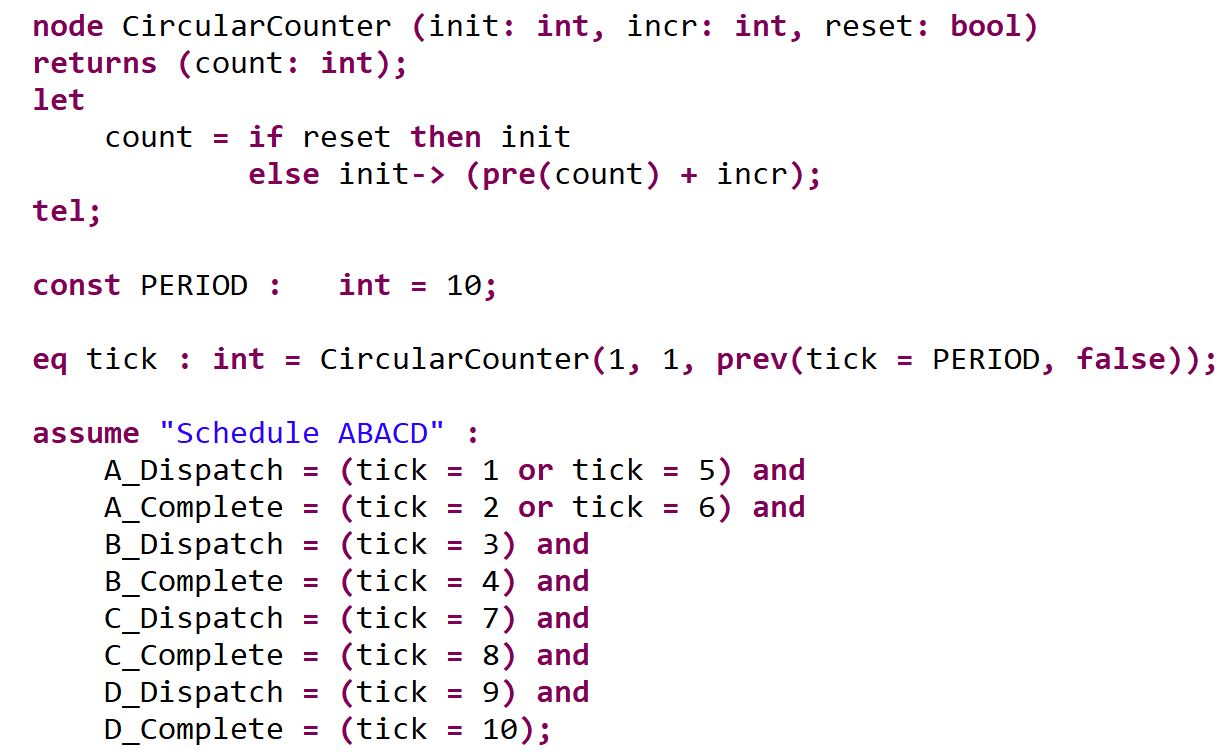
\includegraphics[width=100mm]{schedule.jpg}
\caption{A Model of Schedule in AGREE\label{schedule}}
\end{figure}

%An AGREE model of the schedule $(ABACD)^*$ used in the example is shown in code~\ref{schedule_model}

%\begin{lstlisting}[language=c,frame=single,caption=An AGREE model of a schedule,label=schedule_model]
%node CircularCounter (init: int, incr: int, reset: bool)	
%returns (count: int);
%let
%	count = if reset then init
%		else init-> (pre(count) + incr);
%tel;
%				
%eq tick : int = CircularCounter(1,1,prev(tick=10,false));
%
%assume "Schedule ABACD" :
%	A_dispatch = (tick = 1 or tick = 5) and
%	A_complete = (tick = 2 or tick = 6) and					
%	B_dispatch = (tick = 3) and	
%	B_complete = (tick = 4) and
%	C_dispatch = (tick = 7) and
%	C_complete = (tick = 8) and	
%	D_dispatch = (tick = 9) and
%	D_complete = (tick = 10);			
%\end{lstlisting}	

%The model of a schedule can be simplified to potentially improve the formal verification performance. The thread execution time can be modelled as just one tick. The idle time or communication delay can be abstracted out. For the same example above, a simplified schedule could be  $\sigma' = \{d(A)=(1,0,0)^*, c(A) = (0,1,0)^*, d(B) = (0,1,0)^*, c(B) = (0,0,1)^*\}$. The intuition is that as long as the execution order is preserved, the verfication problem of such a model is equavilent to that of a model directly mapping each base time unit to a tick. 
%	
%\begin{theorem}
%Given an AADL model with two \emph{equavilent} schedules $\sigma$ and $\sigma'$, a property of the model holds under schedule $\sigma$ if and only if it hold under schedule $\sigma'$.
%\end{theorem}
%
%{\bf Proof sketch.} 
%It is possible to show that any counter-example found in the proof of the system property of model with schedule $\sigma$ can be mapped to a counter-example of the proof of the same system property of the same model with schedule $\sigma'$,  and vice versa.  

{\bf external input.} 
Input could arrive at any time instant at an external input port of a thread. However, the thread is activated periodically. To address the asynchrony, we assume that there is a FIFO qeue that stores the input. And the external input arrival rate is properly considered in the schedule, so that all external input data is processed by the thread without causing the buffer overflow. This allows us to simply the timing model by assuming the external input data arrival is coincidental with thread \emph{dispatch} event. That is, for the external input event data ports $I_x$ of thread $A$, 
$$ event(i) \Rightarrow d(A), \forall i \in I_x $$

{\bf AGREE.}
In the assume-gurantee reasoning, the AGREE assumptions of a component work as \emph{assertions}. If an assumption is violated, the system is deemed \emph{inconsistent}. On the other hand, the AGREE guarantees of a component work as \emph{constraints}, which any counterexample has to satisfy.

%As suggested by previous examples, the schedule or execution order has an impact on the system behavior. This differs from other dataflow models, such as Synchronous Dataflow \cite{sdf}, or other variants of Kahn Process Networks \cite{kpn}. It is known 

%{\bf model of execution delay.}
%The thread exeution delay is not directly modelled. Instead, the time slot allocated to a thread in a schedule is modelled by the \emph{distance} between the thread \emph{dispatch} and \emph{complete}. If we assume there is no pre-emption, this modells  the worst case execution time or deadline.

%{\bf model of communication delay.}
%The communication delay is abstracted out. However, in a schedule there is often a time window between the complete event of the one thread and the dispatch event of the next thread. This time window models the %worst case communication delay.

%{\bf AGREE contracts.}

%Our approach to modelling the AADL asynchronous MoC in AGREE is to keep the existing AADL model structure intact and add new AGREE contracts and augument existing contracts. The added contracts model the asynchronous communication between AADL ports. The modification of the exisiting contracts reflcts the interpretation of the contracts under the asychronous AGREE MoC. 

%\begin{figure}[ht!]
%\centering
%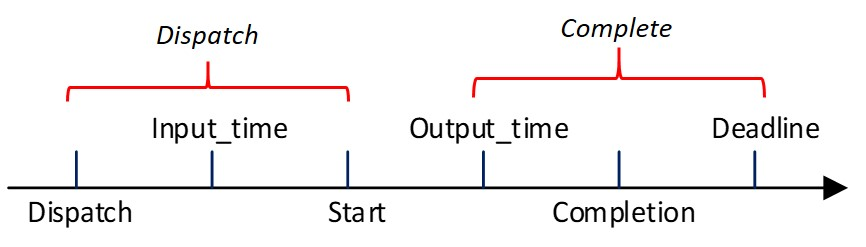
\includegraphics[width=80mm]{aadl_events.jpg}
%\caption{An AADL Model with AGREE Contracts\label{motivation}}
%\end{figure}

%In asynchronous AGREE, the \emph{Execution\_Time} property is modelled by the time interval between the \emph{Dispatch} event and the \emph{Complete} event.
%The assumptions hold at the \emph{Dispatch} event \[Dispatch => Assumption\] , and the guarantees hold at the \emph{Complete} event, i.e. \[Complete => Guarantee\] 
%
%% Assumptions
%We make the following assumptions. The \emph{Input\_Time} property value is unspecified, thus default to dispatch time. The \emph{Output\_Time} property value is unspecified, thus default to the execution completion time. The \emph{Queue\_Size} property value is unspecified, thus default to size one. The \emph{Execution\_Time} property represent a single value, not a real range. The \emph{Dispatch\_Protocol} property value is periodic. The \emph{Timing} property value of each connection is unspecified, thus default to immediate connection. There is no simultaneous read and write access to a queue or buffer (data port). If an event data queue or a data port buffer is empty, the most recent data is used. The \emph{Dequeue} occurs at every dispatch. There is no preemption. There is no propagation delay.
%
%% Modelling
%For an output event data port of a thread, the event and data holds till the thread's next \emph{Complete} event. This is represented by the following AGREE contracts.
%
%\begin{math} 
%not Complete => (event(Port) = prev(event(Port), false))
%\end{math} 
%
%\begin{math}
%not Complete => (true -> (Port = pre(Port)))
%\end{math}  
%
%% Rational
%The output event hold models the latching behavior of an event queue (size one). At the end of execution of a thread, an output event may or may not be raised. However, the AGREE contracts representing the functional requirements only ensures an event is raised only at that exact time instant (i.e. \emph{Complete}). The event is latched so that the target thread, once dispatched, samples the correct result. The consideration for the output data hold is similar.
% 
%% Schedule
%In asynchronous AGREE, a schedule defines the sequential execution order of threads. It is specified by the user. It often come from the actual software execution schedule on the target platform (e.g. seL4 domain schedule). Currently AADL does not define a standard format to specify a schedule. We used AGREE \emph{assumption} on each thread's \emph{Dispatch} and \emph{Complete} event to represent a schedule. For example, \emph{assume "schedule" :			ThreadA\_Dispatch = (Frame = 60) and ThreadA\_Complete = (Frame = 70) and ...}